% Very simple template for lab reports. Most common packages are already included.
\documentclass[a4paper, 11pt]{article}
\usepackage[utf8]{inputenc} % Change according your file encoding
\usepackage{graphicx}
\usepackage{url}

%opening
\title{KTH H16P01 Distributed Systems Basic Course: Routy}
\author{Thorsteinn Thorri Sigurdsson (ttsi@kth.se)}
\date{\today{}}

\begin{document}

\maketitle

\section{Introduction}

In this assignment a link-state routing protocol was implemented in Erlang. A router was implemented which uses Dijkstra's link-state algorithm to generate routing tables that allow different instances of the router to exchange messages.

This is a distributed algorithm that can handle when a node exits and joins. A link state message will be sent that defines the new network topology. A link state message from a node contains information on the node's interfaces, i.e. what other nodes it is connected to. This message is sent to all of the node's neighbors, who then forward it to their neighbors if they haven't seen it before. This way information about the new network topology gets propagated throughout the network.

When a node's view of the network changes it should automatically update its routing tables to construct optimal routing tables for the new network topology (using Dijkstra's algorithm). However, it is worth noting that in this assignment all link state message broadcasts and router updates were done manually, instead of being automatically triggered as they would be in a real life system.

Erlang's \texttt{monitor} feature was used to trigger events on node exits.

\section{Implementation}

Development went rather smoothly. It is worth mentioning that I made a change to the assignment code, by making a node update its own entry in its own map whenever its interfaces were updated (i.e. when receiving an \texttt{add}, \texttt{remove} or \texttt{'DOWN'} message). This way a node will have an entry for itself in its own map. I made this change when initially implementing the solution thinking it was necessary. However tests have shown that it doesn't seem to be.

It also took a little while to understand the implementation, for instance to realize that to make a connection between two routers you needed a bidirectional connection (i.e. add A to B's interfaces and B to A's interfaces).

\section{Evaluation}

Initial testing was done using two Erlang shells, one representing Sweden and another representing Iceland. Both countries had 4 cities (router processes); Stockholm, Lund, Uppsala, Malmo in Sweden and Reykjavik, Akureyri, Isafjordur and Rif in Iceland. Figure \ref{fig:dsbc_a2_routy_sweden_iceland} shows the connections between the different routers.

\begin{figure}[h]
  \begin{center}
    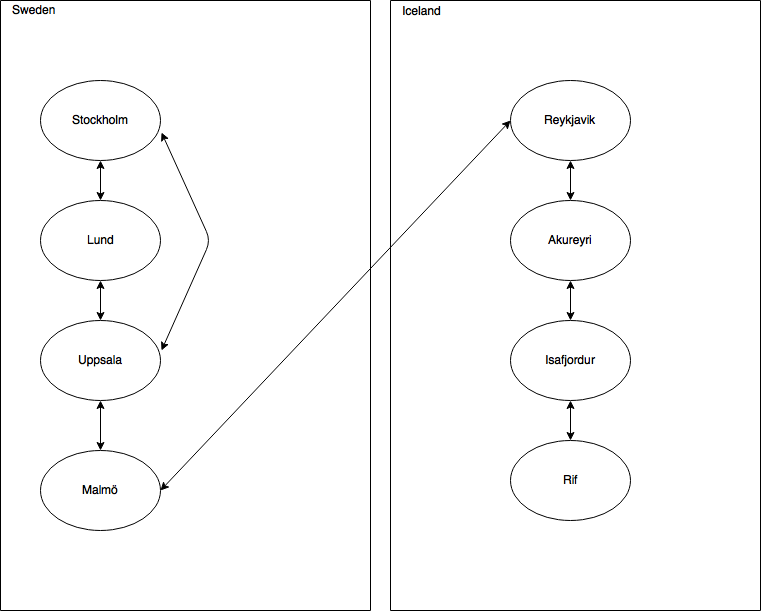
\includegraphics[width=\linewidth]{dsbc_a2_routy_sweden_iceland.png}
    \caption{Structure of the network in the initial test}
    \label{fig:dsbc_a2_routy_sweden_iceland}
  \end{center}
\end{figure}

A message was sent from Stockholm in Sweden to Rif in Iceland. The network is simple, a chain of routers. However, since there is a direct link from Stockholm to Uppsala the shortest path would be to skip Lund and go straight to Uppsala from Stockholm. This would be the correct path. The test was successful and the message went from Stockholm to Uppsala and then from Sweden to Iceland via the Malmö-Reykjavik link.

\begin{verbatim}
(sweden@192.168.1.8)5> 
r1 ! {send, rif, "THIS IS A MESSAGE FROM STOCKHOLM TO RIF"}.
stockholm: routing message (THIS IS A MESSAGE FROM STOCKHOLM TO RIF)
uppsala: routing message (THIS IS A MESSAGE FROM STOCKHOLM TO RIF)
malmo: routing message (THIS IS A MESSAGE FROM STOCKHOLM TO RIF)

(iceland@192.168.1.8)3>
reykjavik: routing message (THIS IS A MESSAGE FROM STOCKHOLM TO RIF)
akureyri: routing message (THIS IS A MESSAGE FROM STOCKHOLM TO RIF)
isafjordur: routing message (THIS IS A MESSAGE FROM STOCKHOLM TO RIF)
rif: received message (THIS IS A MESSAGE FROM STOCKHOLM TO RIF) 
\end{verbatim}

Next another node was added to the test case, Keflavik in Iceland, making a link between Reykjavik-Keflavik-Rif. This would mean that the shortest path from Reykjavik to Rif would now be through Keflavik. The new network topology can be seen in Figure \ref{fig:dsbc_a2_routy_sweden_iceland-keflavik}

\begin{figure}[h]
  \begin{center}
    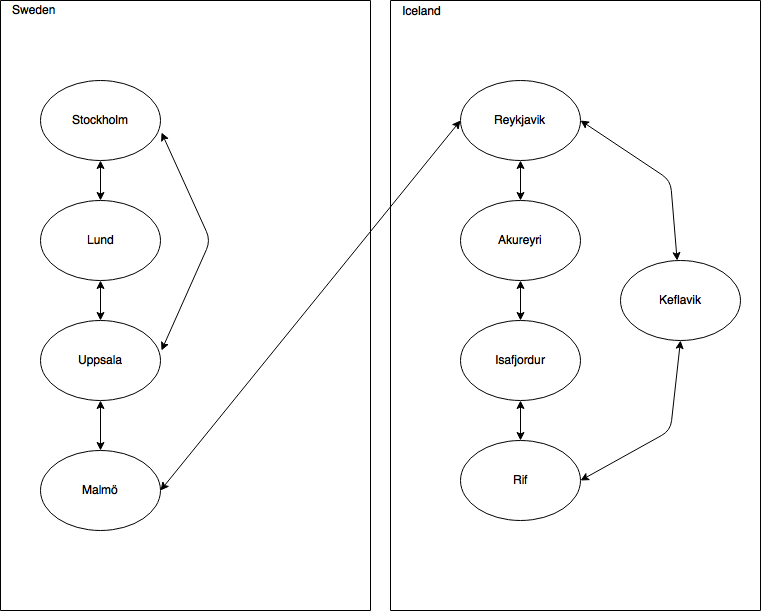
\includegraphics[width=\linewidth]{dsbc_a2_routy_sweden_iceland_keflavik.png}
    \caption{Structure of the network after adding an additional node, Keflavik, in Iceland}
    \label{fig:dsbc_a2_routy_sweden_iceland-keflavik}
  \end{center}
\end{figure}

Again, a message was sent from Stockholm in Sweden to Rif in Iceland. The message took the expected path, going through the Reykjavik-Keflavik-Rif link.

\begin{verbatim}

(sweden@130.229.175.44)4> 
r1 ! {send, rif, "THIS IS A MESSAGE FROM STOCKHOLM TO RIF"}.
stockholm: routing message (THIS IS A MESSAGE FROM STOCKHOLM TO RIF)
uppsala: routing message (THIS IS A MESSAGE FROM STOCKHOLM TO RIF)
malmo: routing message (THIS IS A MESSAGE FROM STOCKHOLM TO RIF)

(iceland@130.229.175.44)3>
reykjavik: routing message (THIS IS A MESSAGE FROM STOCKHOLM TO RIF)
keflavik: routing message (THIS IS A MESSAGE FROM STOCKHOLM TO RIF)
rif: received message (THIS IS A MESSAGE FROM STOCKHOLM TO RIF)

\end{verbatim}

Next Keflavik was taken offline. After sending news of this through the system via link-state messages and having the routers update their routing tables the network should recover. The message should be routed through Reykjavik-Akureyri-Isafjordur-Rif like it was before Keflavik was added. This was successful, the message was routed the expected path.

\begin{verbatim}

(iceland@130.229.175.44)3> routy:stop(r5).
reykjavik: exit received from keflavik
rif: exit received from keflavik
true

... manual calls to broadcast and update ...

(sweden@130.229.175.44)6> 
r1 ! {send, rif, "THIS IS A MESSAGE FROM STOCKHOLM TO RIF"}.
stockholm: routing message (THIS IS A MESSAGE FROM STOCKHOLM TO RIF)
uppsala: routing message (THIS IS A MESSAGE FROM STOCKHOLM TO RIF)
malmo: routing message (THIS IS A MESSAGE FROM STOCKHOLM TO RIF)

(iceland@130.229.175.44)12>
reykjavik: routing message (THIS IS A MESSAGE FROM STOCKHOLM TO RIF)
akureyri: routing message (THIS IS A MESSAGE FROM STOCKHOLM TO RIF)
isafjordur: routing message (THIS IS A MESSAGE FROM STOCKHOLM TO RIF)
rif: received message (THIS IS A MESSAGE FROM STOCKHOLM TO RIF)

\end{verbatim}

\section{Conclusions}

I enjoyed getting the chance to implement Dijkstra's algorithm, an algorithm that has come up several times before in my studies but always in a theoretical context without any practical hands-on exercises.

It was also nice to build an actual resilient distributed system, capable of handling node failures and joins and still function as expected.

Last but not least, this assignment helped improve my skills in Erlang considerably.

\end{document}
